\chapter{Kernel-based Regularization for\\ Consistent Optimal Transport with Empirical Conditional Measures}
\label{chap:ch3}
\section{Introduction}
In this chapter, we demonstrate the application of kernel-based squared Maximum Mean Discrepancy (MMD) regularization to formulate a statistically consistent Optimal Transport (OT) problem between empirical conditional measures.

The need to compare conditional distributions frequently arises in machine learning. For example, supervised learning of probabilistic discriminative models involves comparing the model’s conditional distribution of the label given the input with that learnt from the training data. Another application is in learning implicit conditional generative models. Typically, the observed input covariates in these applications are continuous rather than discrete. Consequently, one may only assume access to samples from the input-label joint distribution rather than having multiple samples for a given input covariate. It is well known that estimating conditionals is a significantly more challenging problem than estimating joints (\citep[Sec. 2]{LiNeykovBalakrishnan}). Hence, it is not straightforward to apply OT between the conditionals as these conditionals are implicitly given via samples from the joint distribution.  This issue is more prominent when the distributions of input covariates in the two joints are not the same, e.g. in medical applications~\citep{hahn2019atlantic} where the distributions of treated and untreated patients differ. In such cases, comparing the joint distributions of input and label is not equivalent to comparing the corresponding conditional distributions.

This chapter addresses this challenging problem of estimating the conditional transport plan between two conditionals, say $s_{Y|X}(\cdot|x)$ and $t_{Y'|X'}(\cdot|x)$ for $x\in \calZ$ (the subspace where conditioned covariate lies), when the samples available are from the joint distributions, $s_{X, Y}, ~t_{X', Y'}$. As motivated above, we do not restrict the variable $x$ to be discrete, nor do we assume that the marginal distributions of the common variable, $s_X$ and $t_{X'}$, are the same. 
Our proposed formulation employs kernelized least-squares terms computed over the joint samples to implicitly match the transport plan's marginals with the empirical conditionals. Under mild assumptions, we prove that our transport cost matches the true expected Wasserstein between the conditionals. With a finite number of samples, $m$, we show that the estimation error of our proposed estimator decays as $O(m^{-1/4})$.

Few prior works have considered special cases of this conditional-OT problem and have proposed formulations to learn conditional transport maps~\citep{Tabak21, Cuturi22}. To the best of our knowledge, our work is the first to formulate OT between conditionals in a general setting modeling the conditional transport plan that also provides a provably consistent estimator for the optimal transport cost. We discuss modeling the conditional transport plan, $\pi^C(y, y'|x)$, through parametric models and propose learning it through the factors: $\pi^C_{Y'|Y,X}(y'|y, x),\ \pi^C_{Y|X}(y|x)$. This gives a three-fold advantage: (i) when dealing with discriminative or conditional-generative models, one can directly choose $\pi^C_{Y|X}(\cdot|x)$ as the discriminative model being learnt, (ii) when implicit generative models are used for modeling the factors, $\pi^C_{Y'|Y,X}(\cdot|y,x)$ can be readily used for inference in conditional generative applications like cell population dynamics (Sec.~\ref{sec:simbio}); when modeled implicitly, the factor $\pi^C_{Y'|Y,X}(y'|y,x)$ enables one-to-many inferences rather than one-to-one inferences provided by transport maps \citep{korotin2023neural}, (iii) the parametric models for these factors can be much simpler than for the joint. For example, in a classification experiment, $\pi^C_{Y'|Y,X}$ can be modeled through a neural network with the final layer as the size of the labels, which is much simpler than modeling the joint over the labels.

We empirically show the utility of our approach in the conditional generative task for modeling cell population dynamics, where we consistently outperform the baselines. Furthermore, we pose the task of learning prompts for few-shot classification as a conditional optimal transport problem. To our knowledge, the existing works on prompt learning have not looked in this direction. We test our novel approach on the benchmark EuroSAT~\citep{helber2019eurosat} dataset and show improvements over~\cite{chen2023plot}, the state-of-the-art baseline for the experiment on prompt learning for few-shot classification.

\section{Contributions}
The main contributions of this chapter are summarized as follows.
\begin{itemize}
\item We propose a novel formulation for OT between conditionals. Compared to the prior works, our formulation is more broadly applicable to settings when samples are provided from the joints and not the corresponding conditionals, where the conditioned variable may be continuous, and its marginals in the two joint distributions may differ.
\item We prove the statistical consistency of the proposed estimator for our conditional-OT formulation. To the best of our knowledge, we are the first to present a consistent estimator for conditional-OT in the general setting.
\item While recent approaches model the OT map \citep{Tabak21,Cuturi22}, we detail different choices for modeling the OT plan, which is advantageous in enabling many-to-one inferences.
\item We begin the empirical evaluation by verifying the correctness of the proposed estimator on synthetic datasets. We further evaluate the proposed approach on downstream applications of conditional generation in modeling cell population dynamics and applications of our conditional-OT divergence in prompt learning for few-shot classification, showing its utility over some of the state-of-the-art baselines.
\end{itemize}

\section{Preliminaries for the Chapter}
We begin by recalling some of the notations and introduce ones specific to this chapter. $x$ denotes the value of the conditioned covariate. $\calZ$ denotes the subspace in which $x$ lies. The measures $s_{Y|X}(\cdot|x),\ t_{Y'|X'}(\cdot|x)\in \calR^+(\calX)$ for $x\in \calZ$. We use the notation $\pi^C(\cdot, \ \cdot|x)$ to denote our conditional transport plan, i.e. transport plan between the conditionals as a function of $x\in \calZ$.
Our problem setting assumes access to sets of joint samples $\calD_m^s = \{(x_1,y_1),\ldots,(x_m,y_m)\}$ and $\calD_m^t=\{(x'_1,y'_1),\ldots,(x'_m,y'_m)\}$ from $s_{X, Y}$ and $t_{X', Y'}$, respectively.

We first recall the definition of MMD from Sec.~\ref{bg:kme}. With a kernel $k$, MMD between $s_0, t_0\in \calR^+(\calX)$ is defined as $\MMD_k(s_0,t_0)= \|\mu_k\left(s_0\right)-\mu_k\left(t_0\right)\|_k,$
where $\mu_k\left(s\right)\equiv \E_{X\sim s}\left[\phi_k(X)\right]$, is the Kernel Mean Embedding of $s$ with $\phi_k$ as the feature map of $k$.  

We also present an important result from \cite{rad}, which is used in showing the statistical consistency of our estimator. A standard tool to quantify the complexity of a class of models is the Rademacher complexity. Rademacher complexity of a model class $F$ computed using IID samples $\{z_i\}_{i=1}^m$ is given by $\mathcal{R}_m(\Pi)=\frac{1}{m}\mathbb{E}\sup\limits_{f\in F} \sum\limits_{i} \epsilon_i f(z_i)$, where the Rademacher variables, $\epsilon_i$'s, are random variables that independently takes values -1 or 1 with equal probability. \citet[Corollary (4)]{rad} presents a bound on the Rademacher complexity of Lipschitz (Definition \ref{defn:f-L}) vector-valued functions, stated as follows.

\begin{restatable}{lemma}{Restated}\label{vecrad}
Restated from \citet[Corollary (4)]{rad}. 
Let $\calH$ denote a Hilbert space and let $F$ be a class of functions $f:\calZ\mapsto \calH$, let $h_i:\calH\mapsto \R$ have Lipschitz norm $L$. Then,
$$\E\sup_{f\in F} \sum_i \epsilon_i h_i(f(x_i))\leq \sqrt{2}L\sum_{i,k} \epsilon_{ik} f_k(x_i),$$
where $\epsilon_{ik}$ is an independent doubly indexed Rademacher sequence, and $f_k(x_i)$ is
the $k$-th component of $f(x_i)$, where $x_i$'s are IID samples.
\end{restatable}

\section{Literature Review}
We discuss the prior works which have attempted to solve the conditional-OT problem in some special cases. ~\cite{Frogner15} present an estimator for the case when the marginals, $s_X$ and $t_{X'}$, are the same and the label $Y$ takes discrete values. Their estimator does not generalize to the case where $Y$ is continuous. Further, they solve individual OT problems at each input $x$ rather than modeling the transport map/plan as a function of $x$. \cite{Bures} proposed \textit{Conditional Kernel Bures (CKB)} divergence for characterizing the discrepancy between conditional distributions. With the assumption that the Kernel Mean Embeddings for the source and target are jointly Gaussian, CKB defines a metric between conditionals. \cite{Bures} do not discuss any (sufficient) conditions for this assumption to hold. Moreover, CKB only estimates the discrepancy between the two conditionals, and it is unclear how to retrieve an optimal transport plan/map with CKB, limiting its applications. \cite{Cuturi22} consider special applications where for each $x\in \calZ$, multiple samples from $s_{Y|X}(\cdot|x), ~t_{Y'|X'}(\cdot|x)$ are available. This approach is referred to as \textit{CondOT}. CondOT learns a transport map as a function of $x$ by solving usual OT problems between $s_{Y|X}(\cdot|x), ~t_{Y'|X'}(\cdot|x)$ individually for each sample $x$. Also, their approach additionally assumes the ground cost is squared-Euclidean. In contrast, we neither assume access to multiple samples from $s_{Y|X}(\cdot|x), ~t_{Y'|X'}(\cdot|x)$ at each $x$ nor make restrictive assumptions on the ground cost. Further, unlike \cite{Cuturi22}, we estimate the transport plan rather than the transport map. The work closest to ours is that of~\cite{Tabak21}. However, there are critical differences between the two approaches, which we highlight as follows. \cite{Tabak21} formulate a min-max adversarial formulation with a KL-divergence-based regularization to learn a transport map. Such adversarial formulations are often unstable, and~\cite{Tabak21} do not present any convergence results. Their empirical evaluation is also limited to small-scale qualitative experiments. Moreover, unlike the estimation bounds proved in our work,~\cite{Tabak21} do not discuss any statistical learning bounds or consistency guarantees. It is expected that such bounds would be cursed with dimensions~\citep{sduot, sliced-uot}. Additionally, our proposed formulation allows us to learn transport plans using implicit models ($\S$~\ref{imp}). Such an approach may not be possible with KL-regularized formulation in~\cite{Tabak21} as training an implicit model involves comparing distributions with potentially non-overlapping support. With these limitations in prior works, we argue that the proposed method is more widely applicable. In Table~\ref{table:relw}, we highlight some of the key features of the proposed conditional-OT (COT) method, comparing it with the related works.
\begin{table*}[t]
  \caption[Summarizing theoretical comparison of the proposed COT formulation with related works.]{Summary of related works and the proposed COT formulation.}
  \label{table:relw}
  % \begin{center}
  \centering
  \setlength{\tabcolsep}{0.3em}
  \small{\begin{tabular}{lcccc}
    \toprule
     Property & Tabak et al. & Luo and Ren & Bunne et al.  & \cellcolor{green!10} Proposed\\
     & [2021] & [2021] (CKB) & [2022] (CondOT) & \cellcolor{green!10}(COT)\\
    \midrule
    Consistent estimator & N/A & N/A & N/A &  \tikzcmark\\
    Implicit modeling choice & \tikzxmark & \tikzxmark & \tikzxmark &  \tikzcmark\\
    Flexible ground cost & \tikzcmark & \tikzxmark & \tikzxmark &  \tikzcmark\\
    With samples from the joint & \tikzcmark & \tikzcmark  & \tikzxmark &  \tikzcmark \\
    \bottomrule
  \end{tabular}}
  % \end{center}
\end{table*}
\section{Proposed Methodology}
This section discusses the proposed conditional-OT (COT) formulation for solving an OT problem between empirical conditional measures. Subsequently, we present the statistical consistency guarantees for estimating the proposed estimator using finite samples and discuss different choices for modeling the transport plan. 
\subsection{Problem Formulation}
We present a series of simplification steps that would take us to the final conditional-OT (COT) formulation that can be estimated using samples from the joints alone. 

We begin by recalling the definition of Kantorovich-OT (Eq. \ref{eqn:kot}) between two given distributions $s_{Y|X}(\cdot|x),\ t_{Y'|X'}(\cdot|x)\in \calR_1^+(\calX)$ for a given $x\in \calZ$.
\begin{align}\label{eqn:indcot}
\bar{W}_{c,1}(s_{Y|X}(\cdot|x), \ t_{Y'|X'}(\cdot|x)) \equiv &\min_{\pi_{Y, Y'|X}(\cdot,\ \cdot|x)\in\mathcal{R}_1^+(\calX\times\calX)}\int_{\calX\times\calX} c\ \textup{d}\pi_{Y, Y'}(\cdot,\ \cdot|x), \\
&\textup{ s.t.}\ \ \pi_{Y|X}(\cdot|x)=s_{Y|X}(\cdot|x), \ \pi_{Y'|X}(\cdot|x)=t_{Y'|X'}(\cdot|x),\nonumber
\end{align}
where $\pi_{Y|X}(\cdot|x)$ and $\pi_{Y'|X}(\cdot|x)$ denotes the marginals of the OT plan, $\pi_{Y, Y'|X}(\cdot,\ \cdot|x)$.
If the cost is a valid metric over $\calX \times \calX$, then the optimal value of Problem~\ref{eqn:indcot} becomes the Wasserstein metric over the measures. While this notion helps in comparing or transporting measures given a specific $x\in\calZ$, in applications like supervised learning~\citep{Frogner15}, one prefers to have a comparison as an expectation over $\calZ$ rather than at a specific $x\in\calZ$. Accordingly, we present the expected Wasserstein distance, $\E_{X^{''}\sim a}\left[\bar{W}_{c,1}\left(s_{Y|X}(\cdot|X^{''}), ~t_{Y'|X'}(\cdot|X^{''})\right)\right]$, with $a$ as a given auxiliary measure, as follows.
\begin{align}\label{eqn:expcot}
 \int_{\calZ}&\min_{\begin{array}{c}\scriptstyle
     \pi_{Y, Y'|X}(\cdot, \ \cdot|x)\in\mathcal{R}_1^+(\calX\times\calX)\ \forall x\in \calZ
\end{array}}\int_{\calX\times\calX} c\ \textup{d}\pi_{Y,  Y'|X}(\cdot, \ \cdot|x) \ \textup{d}a(x), \nonumber\\
&\qquad\quad\qquad\textup{ s.t.}~ \pi_{Y|X}(\cdot|x)=s_{Y|X}(\cdot|x), \ 
\pi_{Y'|X}(\cdot|x)=t_{Y'|X'}(\cdot|x)\ \forall x\in \calZ\nonumber \\
\equiv &\min_{\pi^C_{Y, Y'|X}:\calZ\mapsto\mathcal{R}_1^+(\calX\times\calX)}\int_{\calZ}\int_{\calX\times\calX} c\ \textup{d}\pi^C_{Y, Y'|X}(\cdot, \ \cdot|x)\ \textup{d}a(x), \nonumber\\
&\qquad\quad\qquad\textup{ s.t.}~ \pi^C_{Y|X}(\cdot|x)=s_{Y|X}(\cdot|x),\ \pi^C_{Y'|X}(\cdot|x)=t_{Y'|X'}(\cdot|x)\ \forall x\in \calZ.
\end{align}
In the special case where the auxiliary measure, $a$, is degenerate, Eq.~\ref{eqn:expcot} gives back Eq.~\ref{eqn:indcot}.
The measure $a$ can be taken as the empirical measure over the samples provided.

Henceforth, we analyze the proposed formulation defined in Problem~\ref{eqn:expcot}.
In typical machine learning applications, the conditionals are not explicitly given, and only samples from the joints are available. Estimating the conditionals in Problem~\ref{eqn:expcot} from samples seems challenging because the problem of estimating conditional densities itself has been acknowledged to be a significantly difficult one with known impossibility results (e.g., refer to 
\citet[Sec. (2)]{LiNeykovBalakrishnan}). Hence, some regularity assumptions are necessary for a statistically consistent estimation. Further, even after making appropriate assumptions, the typical estimation errors suffer from the curse of dimensionality (e.g., 
~\citet[Theorem~(2.1)]{Graham2020MinimaxRA}).

On the other hand, estimation of Kernel Mean Embeddings of conditional measures can be performed at rates $O(m^{-1/4})$, where $m$ is the number of samples~\citep{Song2009HilbertSE,gretton}, using samples from the joints alone. This motivates us to enforce the marginal-matching constraints in Problem~\ref{eqn:expcot} by regularizing the corresponding Kernel Mean Embeddings of the measures \citep{Muandet_2017} achieved through the MMD regularization.

More specifically, we exploit the equivalence: $\pi^C_{Y|X}(\cdot|x)=s_{Y|X}(\cdot|x)\ \forall x\in \calZ\iff\left(\mathbb{E}_{X\sim s_{X}}\left[\MMD^2\left(\pi^C_{Y|X}(\cdot|X), ~s_{Y|X}(\cdot|X)\right)\right]=0\right)$ with a reasonable assumption that $s_X(x)>0, \ t_{X'}(x)>0\ \forall\ x\in\calZ$. Using this, Problem~\ref{eqn:expcot} can be relaxed as:
\begin{align}\label{eqn:regcot1}
\min_{\pi^C_{Y, Y'|X}:\calZ\mapsto\mathcal{R}_1^+(\calX\times\calX)}&\int_{\calZ}\int_{\calX\times\calX} c\ \textup{d}\pi^C_{Y, Y'|X}(\cdot,\ \cdot|x)\ \textup{d}a(x) \nonumber\\+ \lambda_1&\int_\calZ\MMD^2\left(\pi^C_{Y|X}(\cdot|x), \ s_{Y|X}(\cdot|x)\right)\textup{d}s_X(x)\nonumber\\
+\lambda_2&\int_\calZ\MMD^2\left(\pi^C_{Y'|X}(\cdot|x), \ t_{Y'|X'}(\cdot|x)\right)\textup{d}t_{X'}(x),
\end{align}
where $\lambda_1,\lambda_2>0$ are regularization hyperparameters. It should be noted that Problem~\ref{eqn:regcot1} is exactly the same as Problem~\ref{eqn:expcot} when $\lambda_1,\lambda_2\rightarrow\infty$.

We now present a key step that simplifies the formulation in terms of samples available from the joints. We know that squared-MMD between the measures is the squared norm of the difference between the corresponding Kernel Mean Embedding vectors (Sec.~\ref{bg:kme}). 
We combine this with the standard result on conditional variance based on the total expectation rule, re-written as $\Big(\E\left[\|G-h(X)\|^2\right]= \E\left[\|G-\E[G|X]\|^2\right] + \E\left[\|\E[G|X] - h(X)\|^2\right]\Big)$. To apply this result for simplifying our formulation, $G$ is taken as the Kernel Mean Embedding of $\delta_Y$ and $h(X)$ denotes the Kernel Mean Embedding of $\pi^C_{Y|X}(\cdot|X)$ to get the following relation, $$\int_{\calZ\times\calX}\MMD^2\left(\pi^C_{Y|X}(\cdot|x), \delta_y\right)\textup{d}s_{X, Y}(x,y)= \int_\calZ\MMD^2\left(\pi^C_{Y|X}(\cdot|x), ~s_{Y|X}(\cdot|x)\right)\textup{d}s_X(x)+v(s),$$
where we have a non-negative term $v(s)$ which is independent of $\pi^C$.


With $\Lambda$ denoting the set of (positive) regularization hyperparameters, $\{\lambda_1, \lambda_2\}$, and $k$ as the kernel used in the definition of the MMD terms, the proposed COT formulation is presented as follows.
\begin{definitionBox}
\vspace{-0.15in}
\begin{align}\label{eqn:regcot2}
\calCW(s_{Y|X},\ t_{Y'|X'}) \coloneqq \min_{\pi^C_{Y, Y'|X}:\calZ\mapsto\mathcal{R}_1^+(\calX\times\calX)}&\int_{\calZ}\int_{\calX\times\calX} c\ \textup{d}\pi^C_{Y, Y'|X}(\cdot,\ \cdot|x)\ \textup{d}a(x) \nonumber\\
+\lambda_1&\int_{\calZ\times\calX}\MMD^2\left(\pi^C_{Y|X}(\cdot|x), \ \delta_y\right)\textup{d}s_{X, Y}(x,y)\nonumber\\
+\lambda_2&\int_{\calZ\times\calX}\MMD^2\left(\pi^C_{Y'|X}(\cdot|x),\ \delta_y\right)\textup{d}t_{X', Y'}(x,y).
\end{align}
\vspace{-0.25in}
\end{definitionBox}

The solution of the COT formulation (Problem~\ref{eqn:regcot2}) is the same as those of Problem~\ref{eqn:expcot} when $\lambda_1,\lambda_2\rightarrow\infty$. This is because the remaining terms are independent of $\pi^C_{Y, Y'|X}$. The advantage of this reformulation is that it can be efficiently estimated using samples from the joints, as we discuss in the next section. It is also worth noting that unlike Problem~\ref{eqn:expcot}, the proposed COT formulation admits a solution even for unnormalized measures $s_{Y|X}\in \calR^+(\calX)$ and $t_{Y'|X'}\in \calR^+(\calX)$.

\subsection{Finite-Sample-based Estimation}
In this section, we discuss estimating the COT formulation (Problem~\ref{eqn:regcot2}) when we only have access to empirical measures supported over finite samples. Since $a$ is a given distribution, we need not estimate the first term in the COT objective with its empirical average. We employ a sample-based estimator for the regularization terms with guarantees based on the following lemma (proved in Appendix~\ref{cot:lemma1}), which shows such estimators to be statistically consistent.
\begin{lemmaBox}
\begin{restatable}{lemma}{lemmaone}\label{lemma}
Assuming $k$ is a normalized characteristic kernel \citep{SriperumbudurFL11}, with probability at least $1-\delta$, we have the following.
\footnotesize{\begin{align*}
\left|\int_{\calZ\times\calX}\MMD^2\left(\pi^C_{Y|X}(\cdot|x), \delta_y\right)~ \textup{d}s_{X, Y}(x, y)-\frac{1}{m}\sum\limits_{i=1}^m\MMD^2\left(\pi^C_{Y|X}(\cdot|x_i), \delta_{y_i}\right) \right|
\le 2\sqrt{\frac{2}{m}\log\left(\frac{2}{\delta}\right)}.
\end{align*}}
\end{restatable}
\end{lemmaBox}
With this, we now present our finite-sample-based estimator for COT (Problem~\ref{eqn:regcot2}).
\begin{align}\label{eqn:empcot2}
\min\limits_{\pi^C_{Y, Y'|X}:\calZ\mapsto\mathcal{R}_1^+(\calX\times\calX)}\int_{\calZ}\int_{\calX\times\calX} c\ \textup{d}\pi^C_{Y, Y'|X}(\cdot, \cdot|x)\ \textup{d}a(x) 
+&\frac{\lambda_1}{m}\sum_{i=1}^m\MMD^2\left(\pi^C_{Y|X}(\cdot|x_i), \delta_{y_i}\right) \nonumber\\
+&\frac{\lambda_2}{m}\sum_{i=1}^m\MMD^2\left(\pi^C_{Y'|X}(\cdot|x'_i), \delta_{y'_i}\right).
\end{align}
We now discuss the statistical consistency of the estimator for conditional-OT in the following theorem, where for simplicity of notations, we assume $\lambda_1=\lambda_2=\lambda$.
\begin{theoremBox}
\begin{restatable}{theorem}{theoremcons}\label{thm1}
Let $\Pi$ be a given model for the conditional transport plans, $\pi^C_{Y,Y'|X}:\calZ\mapsto\mathcal{R}_1^+(\calX\times\calX)$. Let $\widehat{\pi^C_m}, ~\widebar{\pi^C}$ denote optimal solutions over the restricted model $\Pi$ corresponding to (\ref{eqn:empcot2}),\ (\ref{eqn:regcot2}) respectively. Let $\calCW[\widehat{\pi^C_m}],\ \calCW[\widebar{\pi^C}]$ denote the objectives with the Conditional-OT-plan fixed to the corresponding arguments.
\begin{itemize}
\item With probability at least $1-\delta$, $\calCW[\widehat{\pi^C_m}]-\calCW[\widebar{\pi^C_m}]\le2\lambda_1\calR_{m}(\Pi) +2\lambda_2\calR'_{m}(\Pi)+ 6(\lambda_1+\lambda_2)\sqrt{\frac{2}{m}\log{\frac{3}{\delta}}}$, where the Rademacher-based complexity term, $\calR_{m}(\Pi)\coloneqq \frac{1}{m}\E\left[\max\limits_{\pi\in\Pi}\sum_{i=1}^m\epsilon_i\MMD^2\left(\pi_{Y|X}(\cdot|X_i), \delta_{Y_i}\right)\right]$ with $(X_i,Y_i)\stackrel{IID}{\sim} s_{X, Y}$; $\calR'_{m}(\Pi)$, is analogously defined using $(X'_i,Y'_i)\stackrel{IID}{\sim} t_{X', Y'}$ and $\epsilon_i$ is the Rademacher random variable. 
\item In the special case $\Pi$ is a neural-network-based conditional generative model, the kernel employed is universal, normalized, and non-expansive~\citep{pmlr-v168-waarde22a}, and $\lambda_1=\lambda_2=O(m^{1/4})$, with high probability, we have that $\calCW[\widehat{\pi^C_m}]-\calCW[\widebar{\pi^C_m}]\le O(m^{-1/4})$. When $m\rightarrow\infty$, $\widehat{\pi^C_m}$ could become an optimal solution to the original conditional-OT problem (\ref{eqn:expcot}), with $\Pi$ rich enough such that $\exists\widebar{\pi^C_m}\in\Pi\ni\widebar{\pi^C_m}_{Y|X}(\cdot|x)=s_{Y|X}(\cdot|x)$ and $\widebar{\pi^C_m}_{Y'|X}(\cdot|x)=t_{Y'|X'}(\cdot|x) \ \forall x\in \calZ$.
\end{itemize}
\end{restatable}
\end{theoremBox}
The proof is presented in Appendix~$\ref{app:consistency}$. The conditions discussed in the second part are indeed mild because (i) neural conditional generators are known to be universal (\cite[Lemma (2.1)]{Liu2021WassersteinGL},
 ~\citep{pmlr-v125-kidger20a})
 (ii) the popularly used kernels, like the RBF kernel, are universal, normalized, and non-expansive (for a large range of hyperparameters). The proof for the first part of the theorem is an adaptation of classical uniform-convergence-based arguments; however, further bounding the complexity terms in the case of neural conditional generative models is novel, and we derive this using vector contraction inequalities.

\subsection{Modeling the Conditional Transport Plan}\label{modeling}
We now present a pragmatic discussion on modeling the conditional transport plan's function, i.e., choices for $\Pi$. Firstly, we propose modeling the conditional transport plan $\pi^C_{Y, Y'|X}(y, y'|x)$ by modeling its factors: $\pi^C_{Y'|Y, X}(y'|y, x)$ and $\pi^C_{Y|X}(y|x)$. As the factors can be modeled using simpler models, this brings us computational benefits. Furthermore, employing COT with such a factorization enables us to directly choose $\pi^C_{Y|X}(\cdot|x)$ as the label posterior of the model to be learnt in discriminative modeling applications. Moreover, the other factor $\pi^C_{Y'|Y, X}(\cdot|y, x)$ can be readily used for inference in conditional generative modeling ({$\S$~\ref{sec:simbary},~$\S$~\ref{sec:simbio}}).

\subsubsection{Modeling with Explicit Models}\label{expl}
Here, we discuss our modeling choice with explicit probabilistic models when $\calX=\left\{l_1,\ldots,l_n\right\}$ is a finite set. Accordingly, we model the factors $\pi^C_{Y'|Y, X}(y'|y, x),~\pi^C_{Y|X}(y|x)$ with fixed-architecture neural networks, parameterized by $\psi$ and $\phi$ respectively, with the output layer as a softmax over $|\calX|$ labels. The COT estimator (\ref{eqn:empcot2}) in this case simplifies as: 
\begin{align}\label{eqn:expexpcot}\nonumber
&\min\limits_{\psi,\theta}\int_{\calZ}\Bigg(\sum_{i=1,j=1}^{i=n,j=n} c(l_i,l_j)\pi_\psi(l_i|l_j,x)\pi_\theta(l_j|x)\textup{d}a(x) \\&+\lambda_1\frac{1}{m}\sum_{i=1}^m\MMD^2\left(\sum_{j=1}^n\pi_\psi(\cdot|l_j,~x_i)\pi_\theta(l_j|x_i), ~\delta_{y_i}\right)+\lambda_2\frac{1}{m}\sum_{i=1}^m\MMD^2\left(\pi_\theta(\cdot|x'_i), ~\delta_{y'_i}\right)\Bigg).
\end{align}
In discriminative learning applications, the factor $\pi_\theta(\cdot|x)$ can be readily used as a probabilistic classifier (e.g., Sec.~\ref{sec:prompt}).

\subsubsection{Modeling with Implicit Models}\label{imp} 


In applications such as the one discussed in $\S$~\ref{sec:simbio}, it is required to generate samples from $\pi^C_{Y'|Y,X}(\cdot|y,x)$ for inference. In such applications, one would prefer modeling these transport plan factors using implicit generative models.
 

Since the MMD metric, unlike KL-divergence, can be employed to compare measures with non-overlapping support, implicit generative models can be readily employed for modeling our transport plan. More specifically, we model the factors $\pi^C_{Y'|Y, X}(y'|y, x)$, $\pi^C_{Y|X}(y|x)$ with (fixed-architecture) generative neural networks, $\pi_\psi$ and $\pi_\theta$, respectively. We use $\eta,~\eta'\sim \mathcal{N}(0, 1)$ to denote the noise random variables. The $\pi_\theta$ network takes as input $x$ and a random $\eta'$ to produce (random) $y$, to be distributed as $\pi^C_{Y|X}(\cdot|x)$. Likewise, the $\pi_\psi$ network takes as input $y,x$ and a random $\eta$ to produce (random) $y'$, to be distributed as $\pi^C_{Y'|Y,X}(\cdot|y,x)$. We denote the outputs of $\pi_\theta$ by $y(x, \eta'_i;\theta)\ i=1,\ldots,m$ (i.e., samples from $\pi^C_{Y|X}(\cdot|x)$) and we denote outputs of $\pi_\psi$ by $y\left(x, \eta_i, \eta'_i;\theta,\psi\right)\ i=1,\ldots,m$, when inputs  are $y(x, \eta'_i;\theta),x,\eta_i$. We illustrate the overall model in Fig.~\ref{implicit-model}. With this, the COT estimator, with implicit modeling, reads as:
\begin{align}\label{eqn:impcot}
\min\limits_{\theta, \psi}&\int_{\calZ}\Bigg(\frac{1}{m}\sum_{i=1}^m c\left(y(x, \eta'_i;\theta), y\left(x, \eta_i, \eta_i';\theta,\psi\right)\right)\textup{d}a(x) \\+&\frac{\lambda_1}{m}\sum_{i=1}^m\MMD^2\left(\frac{1}{m}\sum_{j=1}^m\delta_{y\left(x_i, \eta_j, \eta'_j;\theta,\psi\right) }, \delta_{y_i}\right) +\frac{\lambda_2}{m}\sum_{i=1}^m\MMD^2\left(\frac{1}{m}\sum_{j=1}^m\delta_{y(x'_i, \eta'_j;\theta) }, \delta_{y'_i}\right)\Bigg).
\end{align}

We note that solving the COT problem learns the factors $\pi^C_{Y'|Y,X}(y'|y,x)$ and $\pi^C_{Y|X}(y|x)$, which can be used for inference purposes. This is in contrast to a typical implicit modeling approach, where one would require samples of $(x,y,y')$ for learning such a model. The unavailability of such triplets (as in {~$\S$~\ref{sec:simbio}}) often limits these traditional generative modeling approaches. On the other hand, COT now allows us to learn such a model without the availability of such triplets, only using (unpaired) samples from $s_{X,Y}$ and $t_{X', Y'}$. This clearly shows the benefits of the proposed approach.

\begin{algorithm}[t]
        \caption[Algorithm for learning the proposed COT estimator with an implicitly modeled conditional transport plan.]{Algorithm for learning the COT estimator with an implicitly modeled conditional transport plan implicit models for a simple regression case.}
        \label{algo-imp}
\begin{algorithmic}[1]
        \Require Implicit models $\pi_{\theta}$ and $\pi_{\psi}$, no. of samples $m$, training samples $(x_i, y_i)|_{i=1}^m$, noise distribution $\eta$, cost function $c$, kernel $k$, $\Lambda$, max epochs.
 
        \While{not converged or max epochs not reached}
        \State Sample $z_i\sim \eta \ \forall i \in [m]$
        \State $y_i(x_i; \theta)=\pi_\theta(\cdot|x_i, z_i) \forall i\in [m]$
        \State Sample $z'_{i}\sim \eta \  \forall i\in [m]$
        \State $y_i (x_i; \theta, \psi) = \pi_\psi(\cdot|y_i (x_i; \theta), x_i, z'_{i}) ;\  \forall i\in [m]$
        \State Compute the COT loss (Simplified case of Eq.~\ref{eqn:impcot})
        \begin{align*} 
        \min_{\theta, \psi}&\frac{1}{m}\sum_{i=1}^m c\left(y_{i}\left(x_i;\theta\right), y_i\left(x_i;\theta,\psi\right)\right) +\lambda\frac{1}{m}\sum_{i=1}^m\MMD_k^2\left(\frac{1}{m}\sum_{j=1}^m\delta_{y_{j}\left(x_i;\theta,\psi\right) }, \delta_{y_i}\right)
        \end{align*}
        \State Update $\theta, \psi$ using gradient descent. 
        \EndWhile   
\end{algorithmic}
\end{algorithm}
\begin{figure}[t]
% \begin{center}
\centering
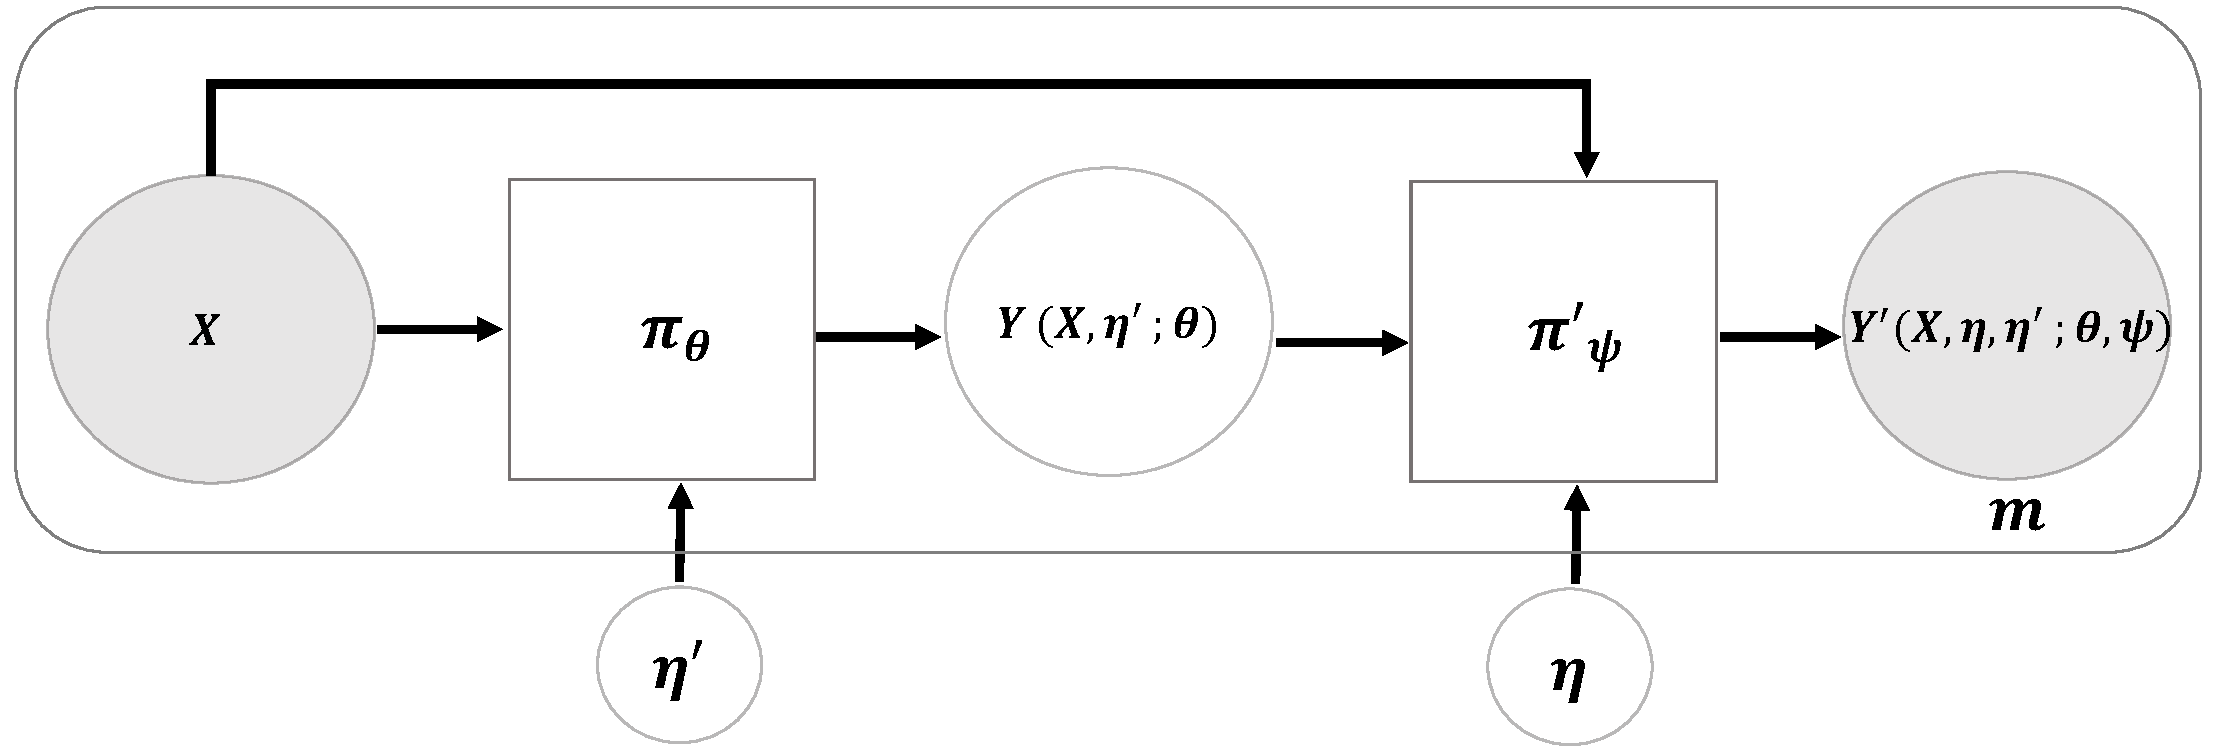
\includegraphics[width=0.6\columnwidth]{chapter-3/images/fig1.pdf}
\caption[Illustration of the proposed factorization and implicit modeling for learning the conditional-OT plan]{Illustration of the proposed factorization and implicit modeling for learning the conditional-OT plan $\pi^C_{Y, Y'|X}(y, y'|x)$ through the factors $\pi_\theta(y|x) \pi_\psi(y'|y, x)$, parameterized by fixed-architecture neural networks (Sec.~\ref{imp}). $\eta, \ \eta'\sim \mathcal{N}(0, 1)$ denotes the noise input to the implicit models.}
\label{implicit-model}
% \end{center}
\end{figure}


\section{Experimental Results}\label{sec:exp}
In this section, we showcase the utility of the proposed COT estimator (\ref{eqn:regcot2}) in various applications.
We choose the auxiliary distribution $a$ as the empirical distribution over the training covariates and use $\lambda_1=\lambda_2=\lambda$ in all our experiments. More experimental details and results are in Appendix~\ref{APP:C}. The code for reproducing our experiments is publicly available at \texttt{https://github.com/atmlr-lab/COT}.
\newline
We begin with detailing our approach to learning the COT estimator for a simple regression case (Appendix~\ref{app-regression}) in Algorithm~\ref{algo-imp}. Next, we empirically verify the correctness of the proposed estimator in synthetically constructed settings where the analytical (closed-form) solutions are known.
\subsection{Verifying Correctness of Estimator}
\subsubsection{Convergence to the True Wasserstein}\label{trueWass}
We learn the implicit networks with the proposed COT loss (\ref{eqn:impcot}), keeping $\lambda$ high enough. With the trained networks, we draw samples $y(x, \eta'_i; \theta)\sim \pi^C_\theta(\cdot|x)$ and $y(x, \eta_i, \eta'_i; \theta, \psi)\sim \pi^C_\psi(\cdot|y(x, \eta'_i; \theta), x)$ , for $i=1,\cdots, m$, and compute the transport cost (first term in \ref{eqn:impcot}) and compare it with 2-Wasserstein between $s_{Y|X}(\cdot|x)$ and $t_{Y'|X'}(\cdot|x))$ at different $x$ values. To verify that our estimate converges to the true Wasserstein, we consider a case where the analytical solution for the Wasserstein distance is known and compare it with our estimate.
\paragraph{Experimental Setup.} We consider two distributions $y \sim \mathcal{N}(4(x-0.5),1)$ and $y' \sim \mathcal{N}(-2(x'-0.5),8x'+1)$ where $x \sim \rm{Beta}(2,4)$ and $x \sim \rm{Beta}(4,2)$ generate $m$ samples from each them. The true Wasserstein distance between them at $x$ turns out to be $(6(x-0.5))^2 + (\sqrt{8x+1}-1)^2$ \cite[Eq. (2.39)]{peyre2019computational}, which we compare our estimate against. We use the RBF kernel and squared-Euclidean distance as our ground cost. The factors $\pi_\theta(\cdot|x)$ and $\pi_\psi(\cdot|y,x)$ are modeled using two 2-layer MLP neural networks.

\begin{figure}[t]
    \centering
    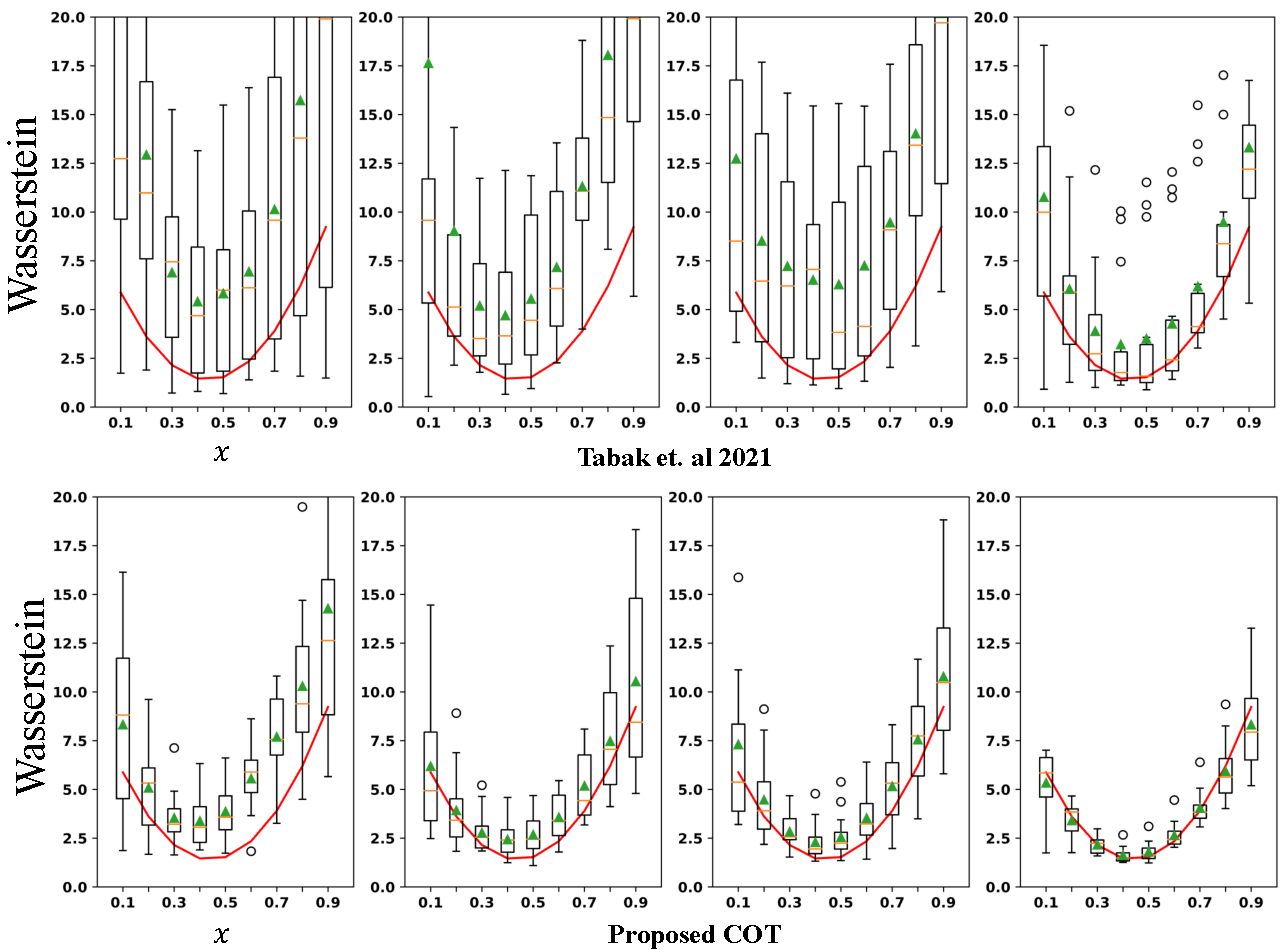
\includegraphics[width=\columnwidth]{chapter-3/images/final-dist-wass.pdf}
    \caption[Evaluation of the proposed COT estimator in terms of convergence to the analytical Wasserstein distance, on increasing the number of samples.]{As $m\in\{100, 200, 400, 800\}$ increases from left to right, we plot the true Wasserstein distance in red and mark the means (in orange) and medians (in green) of the distances estimated using~\cite{Tabak21} and the proposed COT estimator. The statistics are obtained from runs over multiple seeds. The corresponding MSEs are $\{ 245.530, 290.458, 89.715, 27.687\}$ and $\{22.711, 6.725, 8.052, 1.580\}$ respectively. It can be seen that the proposed COT objective converges to the true Wasserstein faster than~\cite{Tabak21}.}
    \label{'fig:correctness'}
\end{figure}
\paragraph{Results.} Fig.~\ref{'fig:correctness'} shows the convergence to the true Wasserstein as $m$ increases. The variance of the estimated values and the mean-squared errors (MSEs) decrease as the number of samples increases. The quadratic nature of the function is also captured with our estimator.
\subsubsection{Convergence to the True Barycenter}\label{sec:simbary}
To further verify our estimator, we show that the barycenter estimated using our conditional transport plans and the true barycenter converge qualitatively and in terms of the Wasserstein distance. 
\paragraph{Experimental Setup.} We take two independent Gaussian distributions $y \sim \mathcal{N}(2(x-0.5),1)$ and $y' \sim \mathcal{N}(-4(x'-0.5),4)$ where  $x \sim \rm{Beta}(2,4)$ and $x' \sim \rm{Beta}(4,2)$.  The analytical solution of the barycenter is calculated as $y_c \sim \mathcal{N}(-x+0.5,2.5)$ \citep{peyre2019computational}.
Recall that the barycenter can also be computed using the optimal transport map (\cite[Remark (3.1)]{pmlr-v97-gordaliza19a}, \citep{interpolationMT}). 
Accordingly, samples from the barycenter, $B_{x_i}$, are obtained using: $\rho y_i+ (1-\rho)y$, where $y \sim \pi_\psi(\cdot|y_i, x_i)$.
\paragraph{Results.} For evaluation, we generate 500 samples from our transport-plan-based barycenter and the true barycenter. We use kernel density estimation (KDE) to plot the barycenters. Figures~\ref{fig:my_label11} and \ref{fig:my_label10} show that the proposed estimate of barycenter closely resembles the analytical barycenter and converges on increasing $m$.
%\cite{flamary2021pot}.
\begin{figure}[t]
    \centering
    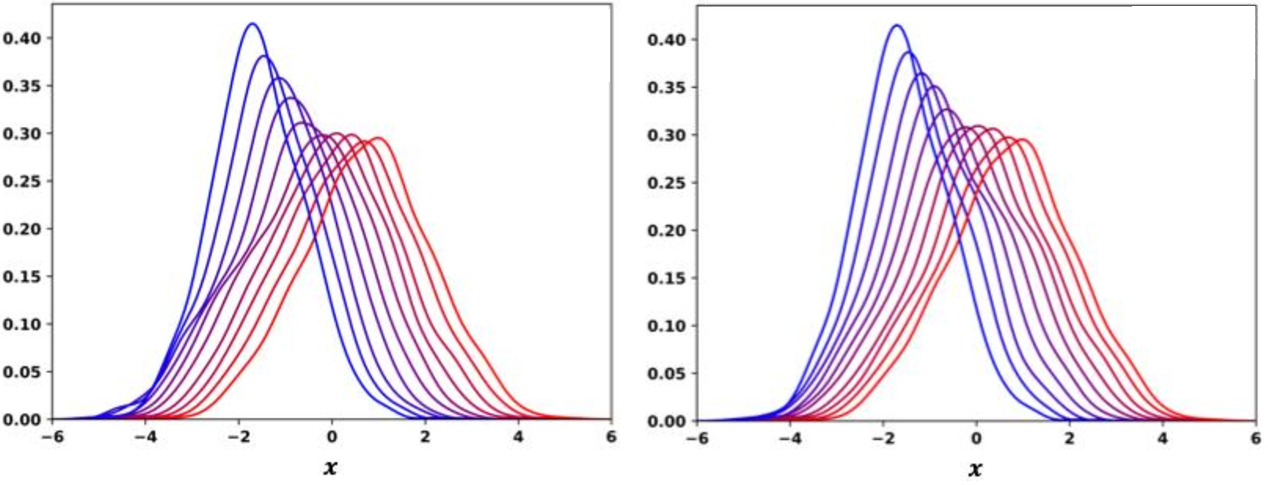
\includegraphics[width=0.6\columnwidth]{chapter-3/images/bary-final-plot.pdf}
    \caption[Qualitative comparison of the barycenters obtained with the proposed COT formulation and the true barycenters.]{Barycenters shown on varying $\rho\in[0, 1]$ with colors interpolated between red (for $s_{Y|X}(\cdot|x)$) and blue (for $t_{Y'|X'}(\cdot|x)$). Left: Conditional barycenter learnt by the proposed COT method. Right: Analytical barycenter.}
    \label{fig:my_label11}
\end{figure}

\begin{figure}[t]
    \centering
    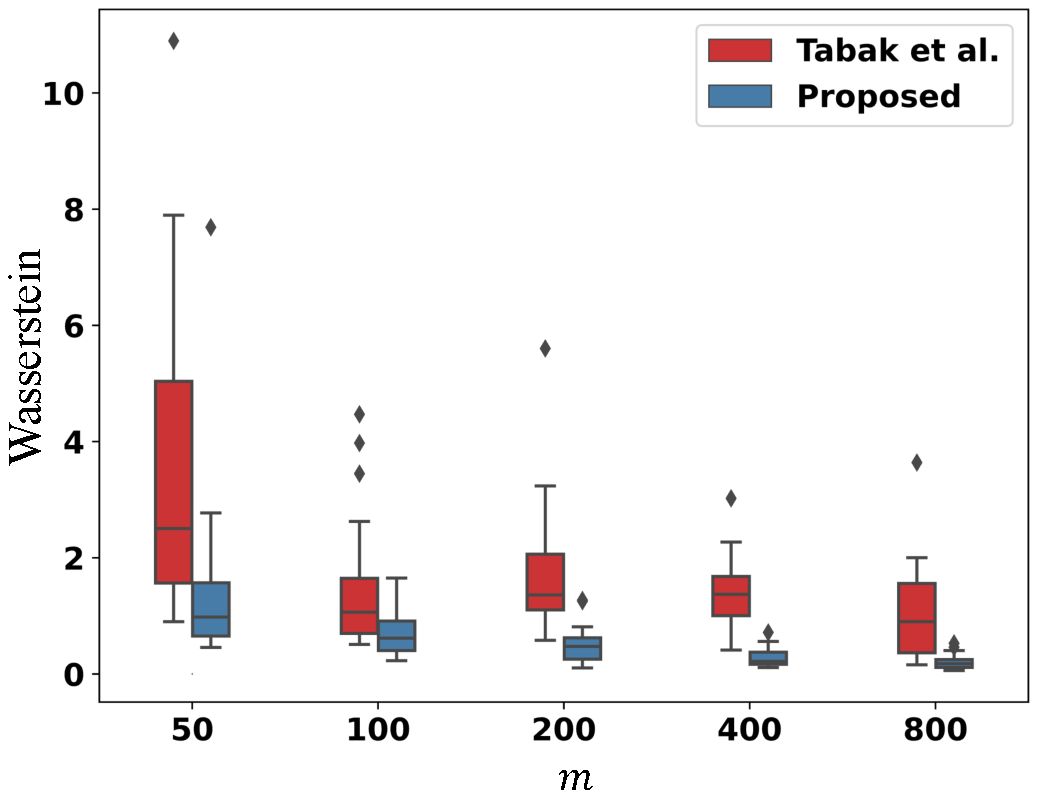
\includegraphics[width=0.4\textwidth]{chapter-3/images/final-bary-wass.pdf}
    \caption[Evaluation of the barycenters obtained with the proposed COT formulation in terms of convergence to the analytical barycenter, on increasing the number of samples.]{For increasing values of $m$, we show box plots of the Wasserstein distance between the learnt barycenter, $B_x$, and the analytical barycenter. The corresponding MSEs are $\{22.399,  3.408, 3.964, 2.534, 1.687\}$ for ~\cite{Tabak21} and $\{4.441, 0.654, 0.353, 0.099, 0.058\}$ for the proposed COT estimator. It can be seen that the proposed COT-based barycenter converges to the true solution faster than~\cite{Tabak21}.}
    \label{fig:my_label10}
\end{figure}
\subsection{Cell-Population Dynamics}\label{sec:simbio}
The study of single-cell molecular responses to treatment drugs is a popular research problem in biology. Existing single-cell-sequencing methods allow one to observe gene expressions of the cells, but do so by destroying them. As a result, one ends up with cells from control (unperturbed) and target (perturbed) distributions without a correspondence between them. The cost minimization term in the OT formulation provides an implicit correspondence, making OT a natural choice for mapping between the source and the target cells \citep{cellot}, which can then be used for predictions on unseen cells. As the drug dosage highly correlates with the predicted cell populations, \cite{Cuturi22} learn such optimal transport maps conditioned on the drug dosage. We apply the proposed COT formulation to generate samples from the distributions over perturbed cells conditioned on the drug dosage given to an unperturbed cell.


\paragraph{Experimental Setup.} Similar to \cite{Cuturi22}, we take the cost function, $c$, as squared-Euclidean. For the MMD regularization, we use the characteristic inverse multi-quadratic (IMQ) kernel.

We consider the dataset used by \cite{Cuturi22} and \cite{cellot} corresponding to the cancer drug \texttt{Givinostat} applied at different dosage levels, $\{x_1=10nM, x_2=100nM, x_3=1000nM, x_4=10000nM\}$. At each dosage level, $x_i$, samples of perturbed cells are given: $y_{i1},\ldots,y_{im_i}$. The total perturbed cells are 3,541. Samples of unperturbed cells are also provided: $y'_1,\ldots,y'_m$ where m is 17,565. Each of these cells is described by gene-expression levels of $n=1000$ highly variable genes, i.e., $y_{ij},\ y'_i\in\R^{1000}$. Following \cite{Cuturi22}, the representations of cells are brought down to 50 dimensions using Principle Component Analysis.
\newline
COT-based Generative modeling: Our goal is to perform OT between the distribution of the unperturbed cells and the distribution of the perturbed cells conditioned on the drug dosage. As the representations of the cells lie in $\calX=\R^{50}$, we choose implicit modeling ($\S$~\ref{imp}) for learning the conditional transport plans. The factor $\pi_\theta$ is taken as the empirical distribution over the unperturbed cells. With this notation, our COT estimator (\ref{eqn:impcot}) simplifies as follows.
\begin{align*}
&\min\limits_{\psi}\frac{1}{4}\sum_{q=1}^4\frac{1}{m}\sum_{i=1}^{m} c\left(y'_{i}, y\left(x_q,\eta_{i};\psi\right)\right)+\lambda_1\frac{1}{4}\sum_{i=1}^4\MMD^2\left(\frac{1}{m}\sum_{j=1}^{m}\delta_{y\left(x_i, \eta_{j};\psi\right) }, \frac{1}{m_i}\sum_{j=1}^{m_i}\delta_{y_{ij}}\right),
\end{align*}
where $y\left(x, \eta_{i};\psi\right)\ i=1,\ldots,m$ are samples from the network $\pi_\psi(\cdot|y'_{i},x)$.

\paragraph{Results.} 

Following \cite{Cuturi22}, we evaluate the performance of COT by comparing samples from the predicted and ground truth perturbed distributions. We report $\ell_2$ (PS), the $\ell_2$ norm between the Perturbation Signatures \citep{Stathias2018DrugAD}, for 50 marker genes with various dosage levels. We also report the MMD distances between the predicted and target distributions with various dosage levels. The distances are reported for in-sample settings, i.e. the dosage levels are seen during training. We compare our performance to the reproduced CellOT~\citep{cellot} and CondOT \citep{Cuturi22} baselines.

We summarize our results in Tables \ref{sample-table-l2} and \ref{sample-table-mmd}. We observe that COT consistently outperforms state-of-the-art baselines CondOT~\citep{Cuturi22} and CellOT~\citep{cellot} in terms of $\ell_2$ (PS) as well as the MMD distances.


\begin{table}[t]
  \caption[Evaluation ($\ell_2$-metric-wise) of proposed COT on the experiment for modeling the cell-population dynamics.]{$\ell_2$ (PS) distances (lower is better) between predicted and ground truth distributions.}
  \label{sample-table-l2}
  \centering
  \begin{tabular}{cccc}
    \toprule
        Dosage   & CellOT & CondOT & \cellcolor{green!10}{Proposed (COT)} \\  
        \midrule
        $10nM$ & 1.2282 & 0.3789 & \cellcolor{green!10}{\textbf{0.3046}}\\
        $100nM$ & 1.2708 & 0.2515 & \cellcolor{green!10}{\textbf{0.2421}}\\
        $1000nM$ & 0.8653 & 0.7290 & \cellcolor{green!10}{\textbf{0.3647}}\\
        $10000nM$ & 4.9035 & 0.3819 & \cellcolor{green!10}{\textbf{0.2607}}\\
        \textbf{Avg.} & 2.067 & 0.4353 &  \cellcolor{green!10}{\textbf{0.2930}}\\
        \bottomrule 
  \end{tabular}
\end{table}

\begin{table}[t]
  \caption[Evaluation (MMD-metric-wise) of proposed COT on the experiment for modeling the cell-population dynamics.]{MMD distances (lower is better) between predicted and ground truth distributions.}
  \label{sample-table-mmd}
  \centering
  \begin{tabular}{cccc}
    \toprule
        Dosage  & CellOT & CondOT & \cellcolor{green!10}{Proposed (COT)}\\  
        \midrule
        $10nM$ & 0.01811 &  0.00654 & \cellcolor{green!10}{\textbf{0.00577}}\\
        $100nM$ & 0.0170 & 0.00555 & \cellcolor{green!10}{\textbf{0.00464}}\\
        $1000nM$ & 0.0154 & 0.01290 & \cellcolor{green!10}{\textbf{0.00647}}\\
        $10000nM$ & 0.1602 & 0.01034 & \cellcolor{green!10}{\textbf{0.00840}}\\
        \textbf{Avg.} & 0.0526 & 0.00883 & \cellcolor{green!10}{\textbf{0.00632}} \\
        \bottomrule 
  \end{tabular}
\end{table}

\subsection{Prompt Learning for Few-Shot Classification}\label{sec:prompt}
\begin{figure}[t]
    \centering
    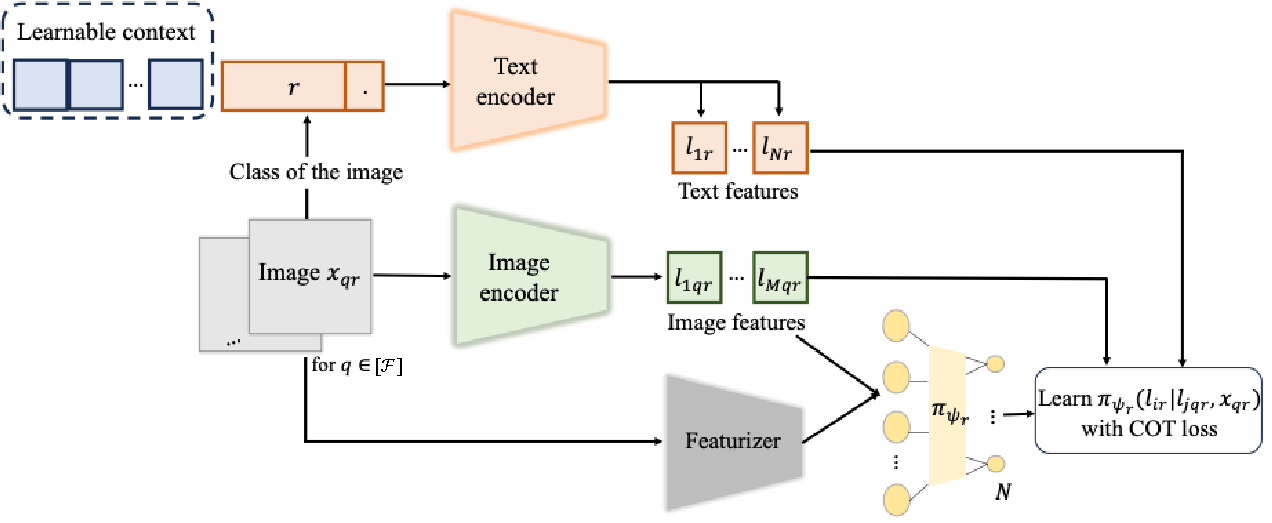
\includegraphics[width=0.9\columnwidth]{chapter-3/images/prompt.pdf}
    \caption[Illustration of the proposed experimental setup for learning prompts for few-shot classification with the proposed COT formulation.]{We pose learning prompts for few-shot classification as the conditional optimal transport problem. The figure shows our neural network diagram for learning conditional optimal transport plans.}
    \label{prompt-diag}
\end{figure}
To show the versatility of our framework, we adapt our estimator for learning prompts for large-scale vision-language models and evaluate the performance in a limited supervision setting. 

The success of vision-language models in open-world visual understanding has motivated efforts which aim to learn prompts to adapt the knowledge from pre-trained models like CLIP~\citep{clip} for downstream tasks since it is infeasible to fine-tune such models due to a large number of parameters \citep{zhou2022cocoop, zhang2021tip, coop,chen2023plot}. Typically, these approaches rely on learning class-specific prompts for each category to better adapt the vision-language model for downstream tasks without the need for fine-tuning. A recent approach, PLOT \citep{chen2023plot}, achieved state-of-the-art results by incorporating an OT-based loss between distributions over the set of local visual features and the set of textual prompt features, each of 1024 dimensions, to learn the downstream classifier. For each image, PLOT computes an OT-based loss between $M (49)$ visual features of the image and $N (4)$ textual prompt features per class. 


 As prompts are shared across images of a class~\citep{chen2023plot}, learning optimal transport plans conditioned on class-level information is expected to improve the downstream performance compared to solving an OT problem separately for each (image, class) pair. Hence, we pose this prompt learning task as a COT problem, where the conditional transport plans are modeled explicitly ($\S$~\ref{expl}).

We learn an explicit model $\pi_{\psi_r}(\cdot|l_{jqr},x_{qr})$ over the $N$ textual prompt features $l_{1r},\ldots,l_{Nr}$ for each class. Here, $x_{qr}$ is the $q^{th}$ image from class $r$ and $l_{jqr}$ is the $j^{th}$ visual feature for image $x_{qr}$. Following PLOT, the distribution over image features given an image is considered uniform and, hence, not modeled as the other factor in the transport plan. Fig.~(\ref{prompt-diag}) depicts the proposed setup. Our formulation for prompt learning for $\mathcal{F}$-shot classification (only $\mathcal{F}$ training images per class) is as follows.
\begin{align}
\min\limits_{\psi_r}&\frac{1}{\calF}\sum_{q=1}^\calF\sum_{i=1,j=1}^{i=N,j=M} c(l_{ir},l_{jqr})\pi_{\psi_r}(l_{ir}|l_{jqr},x_{qr}) \mathbf{v}_j+\lambda_1\MMD^2\left(\sum_{q=1}^\calF \sum_{j=1}^{M}\pi_{\psi_r}(\cdot|l_{jqr},x_{qr})\mathbf{v}_j, \mathbf{u}\right).\label{cot-prompt}
 \end{align}
Following the PLOT setup, $\mathbf{v}, \mathbf{u}$ are uniform weights over the $M(49)$ visual features and the $N(4)$ prompt features, respectively. As the prompts are shared across the images of a class, our MMD-regularization term matches the cumulative marginals to the distribution over prompt features.
\paragraph{Experimental Setup.}
We take the same experimental setup used in CoOp \citep{coop} and PLOT \citep{chen2023plot} for learning prompts and only change the training loss to Eq.~\ref{cot-prompt}. The kernel employed is the characteristic IMQ, and the ground cost is the cosine cost. We follow the common training/evaluation protocol used in CoOp and PLOT and report the mean and standard deviation of the accuracies obtained with 3 seeds.

\paragraph{Results.} In Table \ref{table:prompt}, we report the accuracies on the EuroSAT benchmark dataset \citep{helber2019eurosat} for the number of shots $\mathcal{F}$ as 1, 2, 4 and 8. As the number of shots represents the number of training images per class, learning with lesser $\mathcal{F}$ is more difficult. The advantage of class-level context brought by the proposed COT formulation is evident in this setting. 


\begin{table}[t]
  \caption[Evaluation of proposed COT on the prompt learning experiment for few-shot classification.]{Prompt Learning experiment: Average accuracy (higher is better) on the EuroSAT dataset. The class-level context brought by the proposed COT method allows it to outperform the state-of-the-art PLOT baseline, especially in the challenging case of lesser $\mathcal{F}$.}
  \label{table:prompt}
  \centering
  \setlength{\tabcolsep}{0.5em}
  \begin{tabular}{lccg}
    \toprule
        &  CoOp \citep{coop} & PLOT \citep{chen2023plot} & Proposed (COT) \\  
        \midrule
        $\mathcal{F}=1$ & 52.12 $\pm$ 5.46 & 54.05 $\pm$ 5.95 & \textbf{61.20 $\pm$ 3.65}\\
        $\mathcal{F}=2$ & 59.00 $\pm$ 3.48 & 64.21 $\pm$ 1.90 & \textbf{64.67 $\pm$ 2.37}\\
        $\mathcal{F}=4$ & 68.61 $\pm$ 3.54 & 72.36 $\pm$ 2.29 & \textbf{72.53 $\pm$ 2.60}\\
        $\mathcal{F}=8$ & 77.08 $\pm$ 2.42 & 78.15 $\pm$ 2.65 & \textbf{78.57 $\pm$ 2.38}\\
        \bottomrule 
  \end{tabular}
\end{table}

\section{Conclusion}
Comparing conditionals is often needed in ML applications. With the use of kernel-based MMD regularization, we present COT, the first consistent OT formulation between conditionals.
Remarkably, our framework enables such a comparison solely using samples from (observational) joint distributions.
The main challenge in formulating OT over conditionals is the unavailability of the conditional distributions, which is handled by COT using MMD-based kernelized least-squares terms computed over the joint samples that implicitly match the transport plan’s marginals with the empirical conditionals. This results in the equivalence between Eq.~\ref{eqn:regcot1} and Eq.~\ref{eqn:regcot2} and enables us to model the transport plan with implicit models for applications like those in Sec.~\ref{sec:simbio}.
The statistical efficiency of MMD (Lemma~\ref{cot:lemma1}) helps derive the consistency result (Theorem~\ref{thm1}).
Furthermore, we showcase the utility of the proposed method in downstream applications of cell population dynamics and prompt learning for few-shot classification.

